\begin{figure}
	\centering
	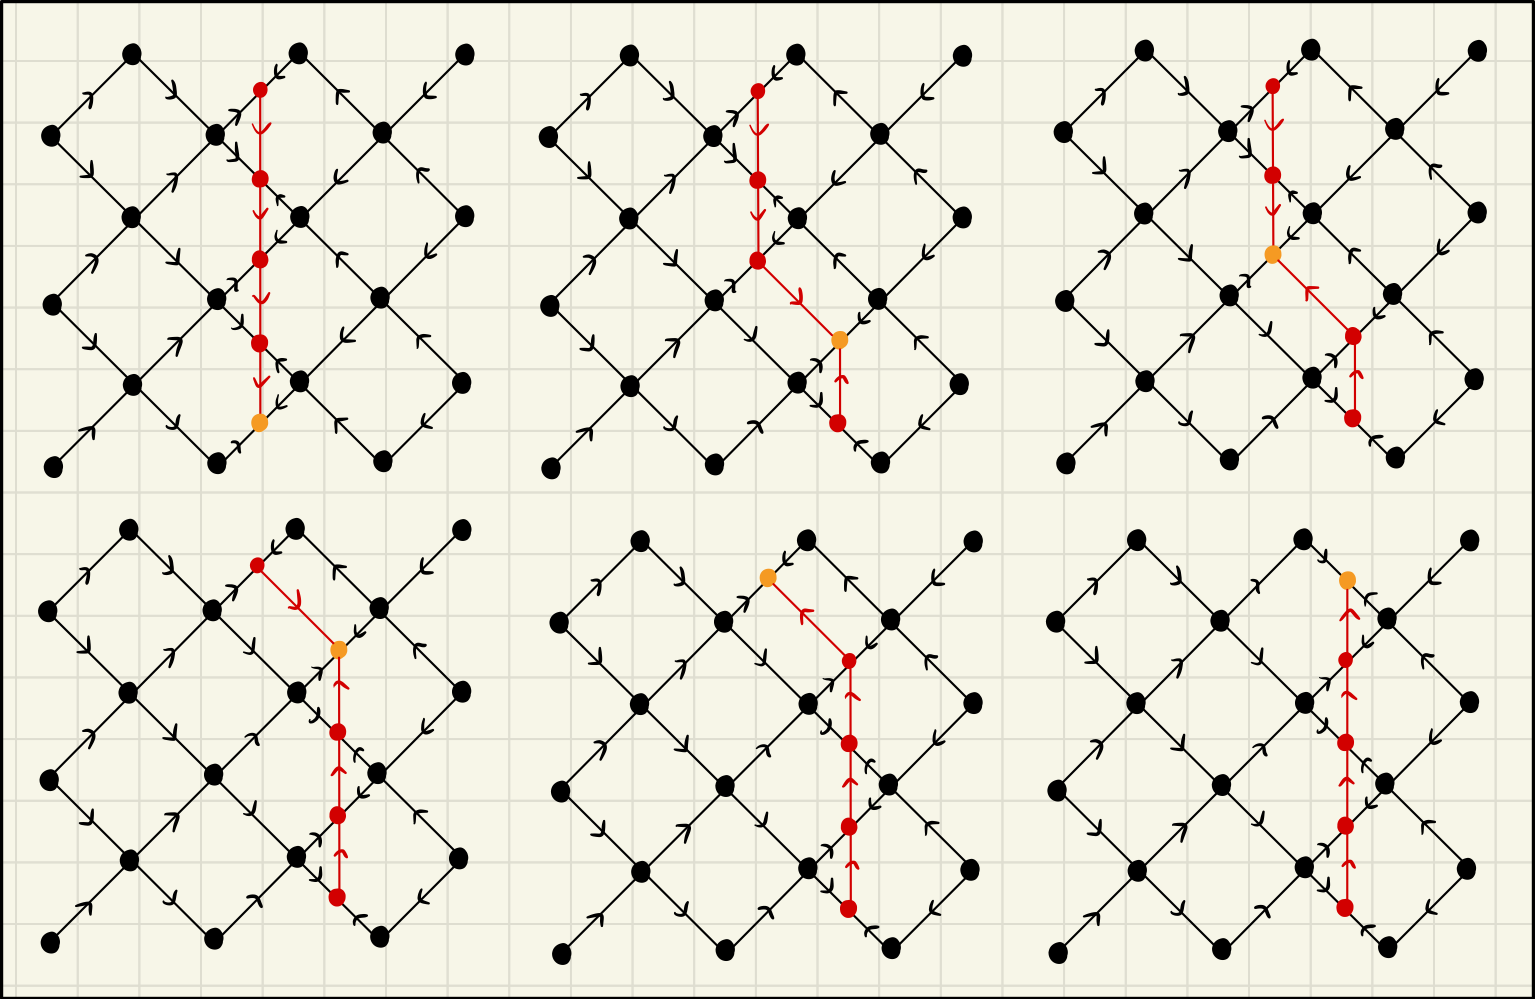
\includegraphics[width=0.9\textwidth]{figures/Tensor_Networks/disoTPS_moving_ortho_surface.jpeg}
	\caption{Two YB-moves are used to shift the orthogonality hypersurface one column to the right. In the last step, the orthogonality center can be moved across the $T$-tensor by contracting the two tensors and performing a QR-decomposition.}
	\label{fig:disoTPS_moving_ortho_surface}
\end{figure}
Most algorithms implemented on disoTPS require an efficient procedure for moving the orthogonality surface, where the error introduced by this procedure should be as small as possible. For isoTPS, the current best procedure is given by the Moses Move, followed by an optional variational optimization. \par
In analogy to the MM we look for a procedure to iteratively shift the orthogonality surface through one column of $T$-tensors as shown in figure \figref{}. A single iteration of this process is shown in figure \figref{}. The two tensors $W_1$ and $W_2$, which are part of the orthogonality hypersurface, are "pulled through" the site tensor $T$, resulting in the updated tensors $T^\prime$, $W_1^\prime$ and $W_2^\prime$. To keep the isometric structure of the network, $T^\prime$ and $W_1^\prime$ must be isometries, while $W_2^\prime$ must be a tensor of norm one (the new orthogonality center). Due to the visual similarity to the Yang-Baxter equation we call this procedure the \textit{Yang-Baxter} (YB) move. One can think of the YB move $W_1W_2T \approx T^\prime W_1^\prime W_2^\prime$ as a constrained optimization problem
\begin{equation}
	\left(T^\prime, W_1^\prime, W_2^\prime\right) = \underset{T^\prime,W_1^\prime,W_2^\prime}{\text{argmin}}\left\lVert W_1W_2T - T^\prime W_1^\prime W_2^\prime\right\rVert,
\end{equation}
\begin{equation}
	T^{\prime\dagger}T^\prime = \id, \quad W_1^{\prime\dagger}W_1^\prime = \id, \quad \left\lVert W_2^\prime \right\rVert = 1,
\end{equation}
where the contraction of $W$- and $T$-tensors is performed as shown in figure \figref{}. \par
\begin{figure}
	\centering
	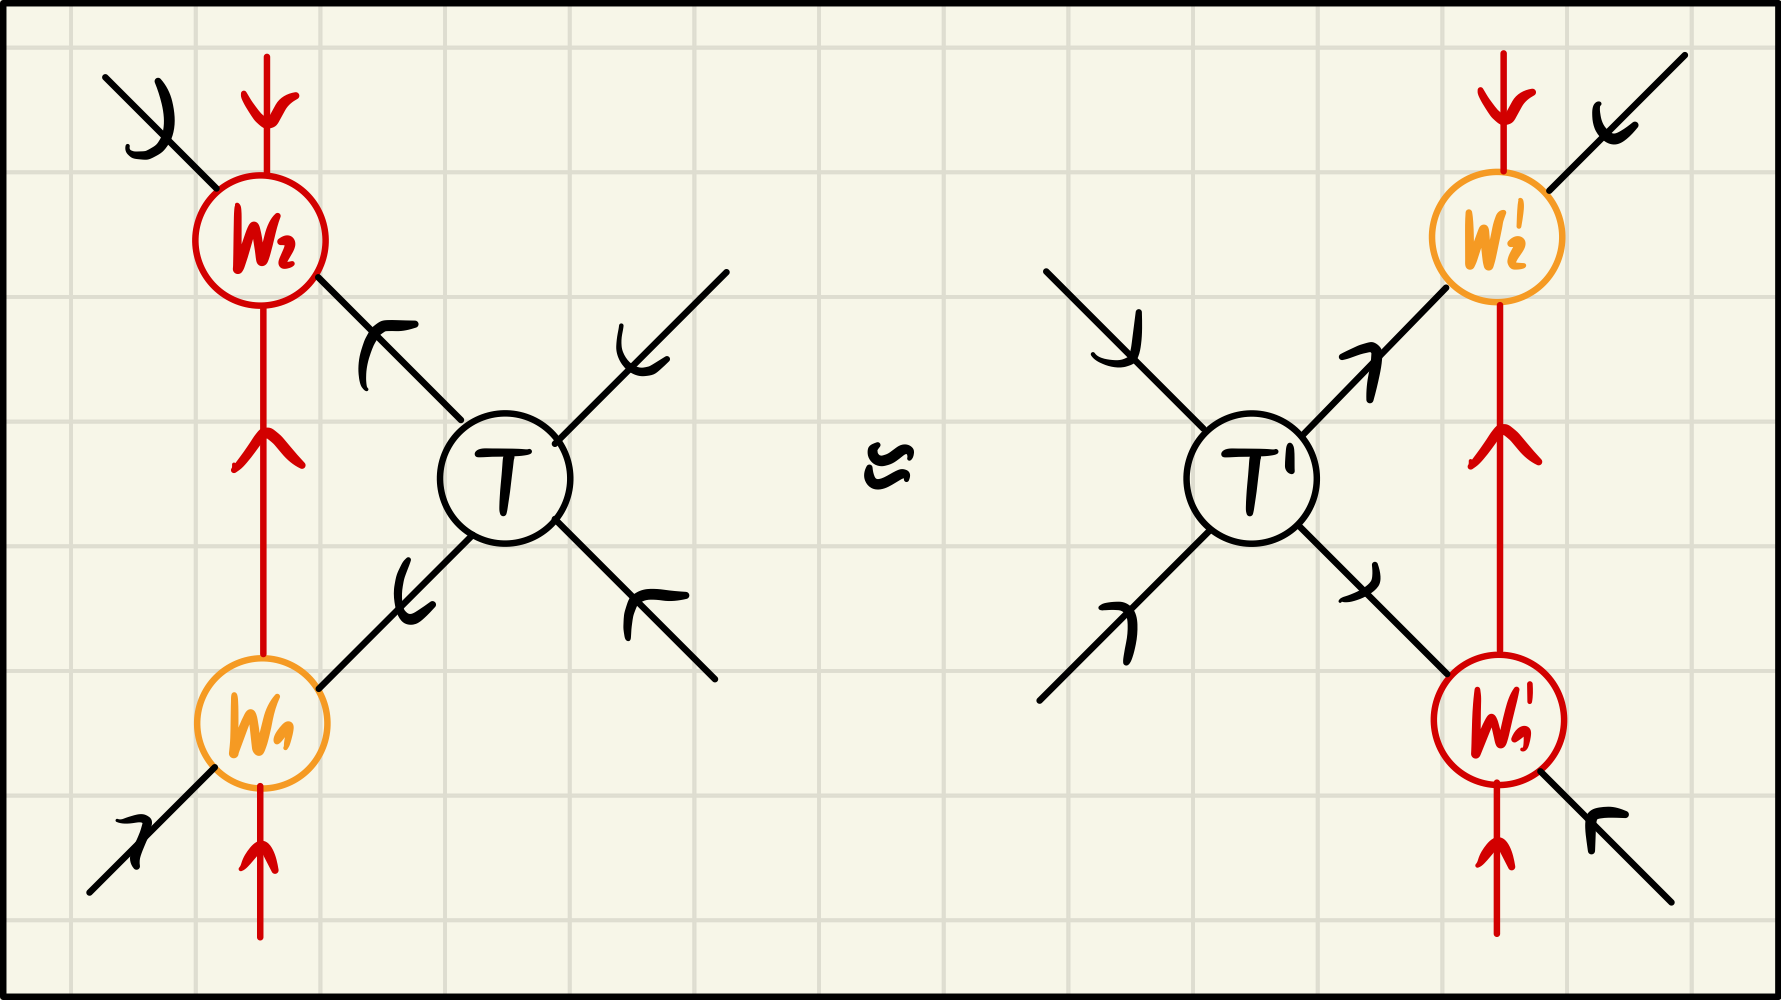
\includegraphics[width=0.9\textwidth]{figures/Tensor_Networks/YB_move_closeup.jpeg}
	\caption{The Yang-Baxter (YB) move is the procedure of "pulling" two auxillary tensors $W_1$ and $W_2$ through a site tensor $T$.}
	\label{fig:disoTPS_YB_move_closeup}
\end{figure}
In the following, we present two explicit algorithms for performing the YB move. The first algorithm is a variational optimization based on the Evenbly-Vidal algorithm, the second algorithm is a tripartite decomposition with disentangling similar to the tripartite decomposition used in the MM. In section \ref{} we will compare the two algorithms.